\documentclass{llncs}


\usepackage{hyperref}
\usepackage{graphicx}
\usepackage{multirow}
\usepackage[misc,geometry]{ifsym}

%\usepackage{amsmath}
%\usepackage{amsfonts}
%\usepackage{amssymb}
%\usepackage{epstopdf}
%\usepackage{epsfig}


%\usepackage{url}
%\urldef{\mailsa}\path|i.surmin@gmail.com, avbk@mail.ru, bastrakov@vmk.unn.ru,  |
%\urldef{\mailsb}\path|evgeny.efimenko@gmail.com, arkady.gonoskov@gmail.com, meerov@vmk.unn.ru|


\begin{document}

\mainmatter 

\title{Solving GENOPT problems \newline with the use of ExaMin solver}
\author{Konstantin Barkalov \Letter \and Alexander Sysoyev \and \\ Ilya Lebedev \and Vladislav Sovrasov \\
\email{ \{konstantin.barkalov,alexander.sysoyev,ilya.lebedev,\\vladislav.sovrasov\}@itmm.unn.ru}}

%\author{Konstantin Barkalov \Letter \and Alexander Sysoyev \and \newline Ilya Lebedev \and Vladislav Sovrasov \email{[konstantin.barkalov,alexander.sysoyev,ilya.lebedev,\newline vladislav.sovrasov]@itmm.unn.ru}}



%\author{Konstantin Barkalov \Letter \and Alexander Sysoyev \and Ilya Lebedev \and Vladislav Sovrasov \email{[konstantin.barkalov,alexander.sysoyev,ilya.lebedev,\newline vladislav.sovrasov]@itmm.unn.ru}}

%\author{Konstantin Barkalov ( \Letter~\email{konstantin.barkalov@itmm.unn.ru})  \and \\ Alexander Sysoyev (\email{alexander.sysoyev@itmm.unn.ru}) \and \\ Ilya Lebedev (\email{ilya.lebedev@itmm.unn.ru})  \and \\ Vladislav Sovrasov (\email{vladislav.sovrasov@itmm.unn.ru}) }

\institute{Lobachevsky State University of Nizhny Novgorod, Nizhny Novgorod, Russia}



\maketitle

\begin{abstract}

This paper describes an algorithm for solving multidimensional multiextremal optimization problems. This algorithm uses Peano-type space-filling curves for dimension reduction. It has been used for solving problems at GENeralization-based
contest in global OPTimization (GENOPT). Computational experiments are carried out on 1800 multidimensional problems.

\keywords global optimization, multiextremal functions, space-filling curves, mixed global-local algorithm, GENOPT.

\end{abstract}

\section{Introduction}
A well-known approach to the investigation and comparing of the multiextremal optimization algorithms is based on testing these methods by solving a set of test problems, chosen randomly from some specially designed class. Each test problem can be considered as a particular instance of a random function generated by a special generator. Application of multiextremal optimization algorithms to large sets of such functions allows estimating the characteristics of the methods and evaluating the efficiency of each particular algorithm.

Among such generators for the one-dimensional problems, there are samples from Fourier series proposed by Hill \cite{Hill}. A generator proposed by Shekel \cite{Shekel} generates another well-known class of the one-dimensional test problems. For the investigation of various one-dimensional algorithms using the samples of the functions generated by Hill and Shekel generators Globalizer software has been developed. A comprehensive description of the capabilities of this system and the examples of its application are given in \cite{Strongin2000}. Note also that Hill and Shekel functions have been successfully used in the construction of one-dimensional constrained problems (with controlled measure of the feasible domain) \cite{Barkalov2002}. 

A generator for a random sampling of two-dimensional test functions has been proposed in \cite{Grishagin1978}. A generator for the functions of arbitrary dimensionality with known positions of the local and global minima (GKLS generator) has been proposed in \cite{Gaviano}. Its application for the studying of some multidimensional algorithms has been described in \cite{Kvasov2003,Sergeyev2013}.

Approach to the comparison of the algorithms by solving a set of test problems has been used by the organizers of GENeralization-based contest in global OPTimization (GENOPT). The functions to be optimized are broadly divided into three function families: GKLS, conditioned transforms of classical benchmarks (Rosenbrock (unimodal, narrowing bending valley), Rastrigin (strongly multimodal), Zakharov (unimodal)), and a composition of classical benchmarks. In their turn, each family is subdivided into six function types, which differ by their analytical definition and by the number of dimensions. The functions belonging to the same type share the majority of properties and can be assumed to have the same difficulty. Finally, every function type of every family is realized into an unlimited number of function instances which differ by some randomly generated parameters. In particular, every instance will have a randomly generated offset $c\in[-1,1]$ added to the function’s output in order to make the global minimum value unpredictable. A detailed description of the competition problems can be found at the website \url{http://genopt.org}.

An efficient approach for solving global optimization problems has been developed under the supervision by prof. R.G. Strongin at Lobachevsky State University of Nizhni Novgorod \cite{Sergeyev1994} -- \cite{Barkalov2016}. Within the framework of this approach, solving multidimensional global optimization problems is reduced to solving a set of the corresponding one-dimensional ones. The corresponding dimension reduction is based on the use of Peano space-filling curves (also called \textit{evolvents}), unambiguously mapping the unit interval of the real axis onto a hypercube, as well as the generalization of these ones, which can be applied to solving the problems using the multiprocessor systems. The proposed algorithms have been implemented in ExaMin solver applied to solving the problems within GENOPT competition. In the present work, a brief description of the global optimization algorithm applied and of its modifications are given, and the results of the computational experiments with the problems of the competition are presented.

\section{Problem statement}

Let us consider the problem of search for a global minimum of an $N$-dimensional function $\varphi(y)$ within a hyperinterval $D$
\begin{eqnarray}\label{eq:1}
& \varphi(y^\ast)=\min{\left\{\varphi(y):y\in D\right\}},\\
& D=\left\{y\in R^N: a_i\leq y_i \leq b_i, 1\leq i \leq N\right\}. \nonumber
\end{eqnarray}

Let us assume that the function $\varphi$ satisfies the Lipschitz condition with an a priori unknown constant $L$
\[
\left|\varphi(y_1)-\varphi(y_2)\right|\leq L\left\|y_1-y_2\right\|,\; y_1,y_2 \in D,\; 0<L<\infty.
\]

In this study, we will use the approach based on the idea of dimension reduction by means of a Peano curve $y(x)$, which continuously and unambiguously maps the unit interval [0,1] onto the $n$-dimensional cube
\[
\left\{y\in R^N: -2^{-1}\leq y_i \leq 2^{-1}, 1 \leq i \leq N\right\}=\left\{y(x):0\leq x \leq 1 \right\}.
\]
%new text begin
Problems of numerical construction of Peano-type space filling curves and the corresponding theory are considered in detail in \cite{Strongin2000}, \cite{Sergeyev2013}.  
%new text begin
Here we will note that a numerically constructed curve is $2^{-m}$ accurate approximation of the theoretical Peano curve in $L_\infty$ metric, where $m$ is an evolvent construction parameter. Examples of the evolvent with different $m$ in two dimensions are given in Fig.~\ref{fig:0}.

\begin{figure}
\begin{minipage}{0.32\linewidth}
\center{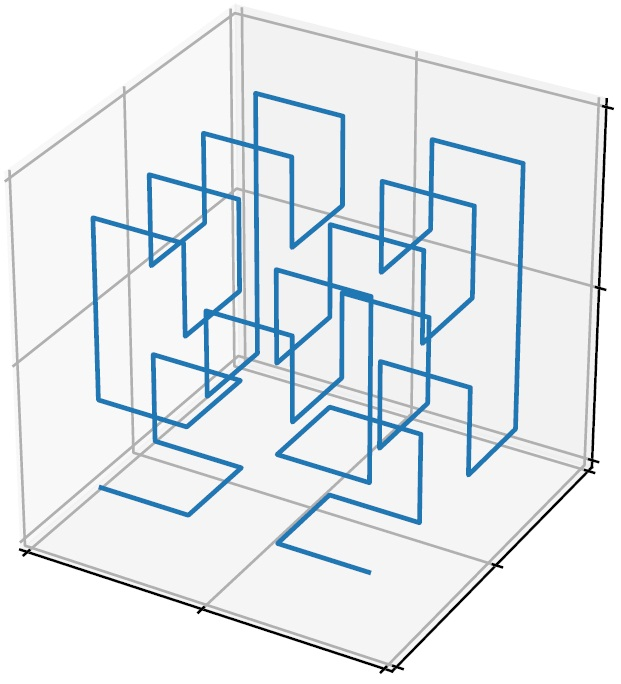
\includegraphics[width=1.0\linewidth]{fig1a.JPG} \\ (a)}
\end{minipage}
\hfill
\begin{minipage}{0.32\linewidth}
\center{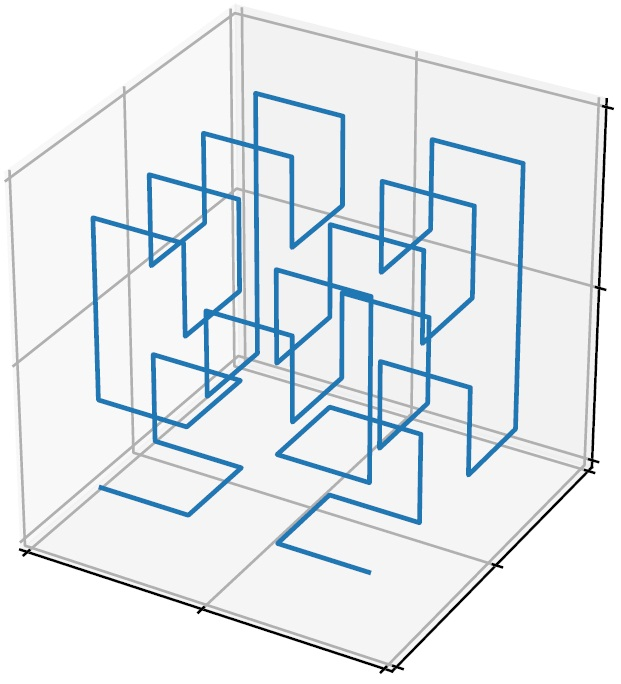
\includegraphics[width=1.0\linewidth]{fig1b.JPG} \\ (b)}
\end{minipage}
\begin{minipage}{0.32\linewidth}
\center{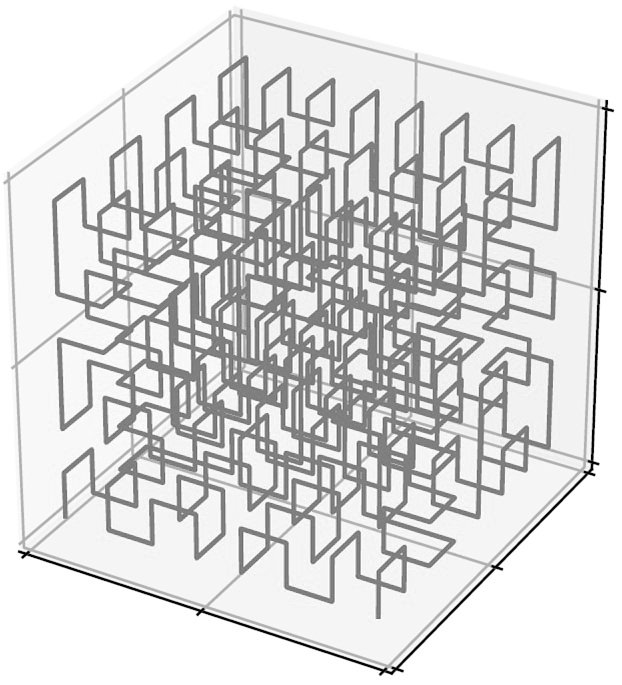
\includegraphics[width=1.0\linewidth]{fig1c.JPG} \\ (c)}
\end{minipage}
\caption{Evolvents in two dimensions with (a) $m=3$, (b) $m=4$ and (c) $m=5$}
\label{fig:0}
\end{figure}


By using this kind of mapping it is possible to reduce the multidimensional problem~(\ref{eq:1}) to a univariate problem
\[
\varphi(y^\ast)=\varphi(y(x^\ast))=\min{\left\{\varphi(y(x)): x\in[0,1]\right\}}.
\]
An important property of such mapping is preservation of boundedness of function relative differences  (see \cite{Strongin2000,Sergeyev2010}): if the function $\varphi(y)$ in the domain $D$ satisfies the Lipschitz condition, then the function $\varphi(y(x))$ on the interval $[0,1]$ will satisfy a uniform H{\"o}lder condition
\[
\left|\varphi(y(x_1))-\varphi(y(x_2))\right|\leq H\left|x_1-x_2\right|^{1/N},
\]
where the H{\"o}lder constant $H$ is linked to the Lipschitz constant $L$ by the relation
\[
H=2L\sqrt{N+3}.%,\;\; d=\max{\left\{b_i-a_i:1\leq i \leq N\right\}}.
\]

Therefore, it is possible, without loss of generality, to consider minimization of univariate function
\[
f(x)=\varphi(y(x)), \;\; x\in[0,1],
\]
satisfying the H{\"o}lder condition.



\section{Global search algorithm}\label{sec:1}

The considered algorithm for solving this problem (here, according to \cite{Strongin2000}) involves constructing a sequence of points $x^k$, where the values of minimized function $z^k = f(x^k)=\varphi(y(x^k))$ are calculated. Let us call the process of calculating the function value (including the construction of an image $y^k=y(x^k)$) the ``trial'', and the pair $(x^k, z^k)$, the ``trial result''. The set of pairs $\left\{(x^k, z^k)\right\}, 1\leq k\leq n,$ makes up the search data collected using the method after carrying out $n$ steps. The rules that determine the work of the global search algorithm are as follows.

At the first iteration of the method the trial is carried out at an arbitrary internal point $x^1$ of the interval $[0,1]$. The point of trial at the next iteration $(k+1)$ is determined according to the rules presented below.

Rule 1. Renumber points of the set
\[
X_k=\{x^1,\dots,x^k\}\cup\left\{0\right\}\cup\left\{1\right\},
\]
which includes boundary points of the interval $[0,1]$ and the points of the previous trials, with subscripts in increasing order of coordinate values, i.e.,
\[
0=x_0<x_1<\dots <x_k<x_{k+1}=1.
\]

Rule 2. Supposing that  $z_i=f(x_i)=\varphi(y(x_i)), \; 1\leq i \leq k$, calculate values 
\begin{equation}\label{eq:11}
\mu = \max_{2\leq i \leq k}\frac{\left|z_i-z_{i-1}\right|}{\Delta_i},
\end{equation}
\[
M = \left\{
   \begin{array}{lr}
     r\mu, & \mu > 0,\\
     1, & \mu = 0,
   \end{array}
\right.
 \]
where $r>1$ is a preset parameter of the method, and $\Delta_i=\left(x_i-x_{i-1}\right)^{1/N}$.

Rule 3. Calculate a \textit{characteristic} for every interval $(x_{i-1}, x_i), \; 1\leq i \leq k+1,$   according to the following formulae
\[
R(1)=2\Delta_1-4\frac{z_1}{M},
\]
\begin{equation}\label{eq:14}
R(i)=\Delta_i+\frac{(z_i-z_{i-1})^2}{M^2\Delta_i}-2\frac{z_i+z_{i-1}}{M},1<i<k+1,
\end{equation}
\[
R(k+1)=2\Delta_{k+1}-4\frac{z_k}{M}.
\]

Rule 4. Find interval $(x_{t-1},x_t)$ with the maximum characteristic
\begin{equation}\label{eq:141}
R(t)=\max{\left\{R(i): 1 \leq i \leq k+1\right\}}.
\end{equation}

Rule 5. Carry out a trial at the point $x^{k+1}\in(x_{t-1},x_t)$, calculated using the following formulae
\[
x^{k+1} = \frac{x_t+x_{t-1}}{2}, \textrm{ if } t=1 \textrm{ or } t=k+1,
\]
\begin{equation}\label{eq:142}
x^{k+1} = \frac{x_t+x_{t-1}}{2} - \mathrm{sign}(z_t-z_{t-1})\frac{1}{2r}\left[\frac{\left|z_t-z_{t-1}\right|}{\mu}\right]^N, \textrm{ if } 1<t<k+1.
\end{equation}

The algorithm terminates if the condition $\Delta_t<\epsilon$ is satisfied; here $\epsilon>0$ is the preset accuracy. As the \textit{current estimate} of an optimum at the step $k$ we accept the value 
\begin{equation}\label{eq:phistar}
\varphi_k^\ast=\min_{1\leq i \leq k}z^i,
\end{equation}
and the vector 
\[
y_k^\ast=\arg \min_{y \in \{ y^1,...,y^k\} }\varphi(y).
\]

%new
This \textit{global search algorithm} (GSA) was developed in the framework of information - statistical approach (see \cite{Strongin2000}). From this point of view the normalized characteristics $R(i)$ from (\ref{eq:14}) can be considered as probabilities of locating the global minimum within the interval  $(x_{i-1},x_i), 1\leq i \leq k+1$. Thus, at each iteration a new trial point is selected inside the interval, which has the greatest probability of finding the global minimum.
At the same time, use of running estimates (\ref{eq:11}) of Lipschitz constant $L$ allows us to apply GSA to the problems with a priori unknown values of $L$. 

Let us illustrate the work of GSA for minimization of a multiextremal function of two variables generated by GKLS generator \cite{Gaviano}. %function No 4, simple
The experiment used the method parameters $r=3$, $\epsilon=10^{-3}$, and the evolvent construction parameter $m=10$. Fig.~\ref{fig:1} shows the level lines of the function and the points of 421 trials carried out by the method before the required accuracy was obtained.
\begin{figure}
	\center
  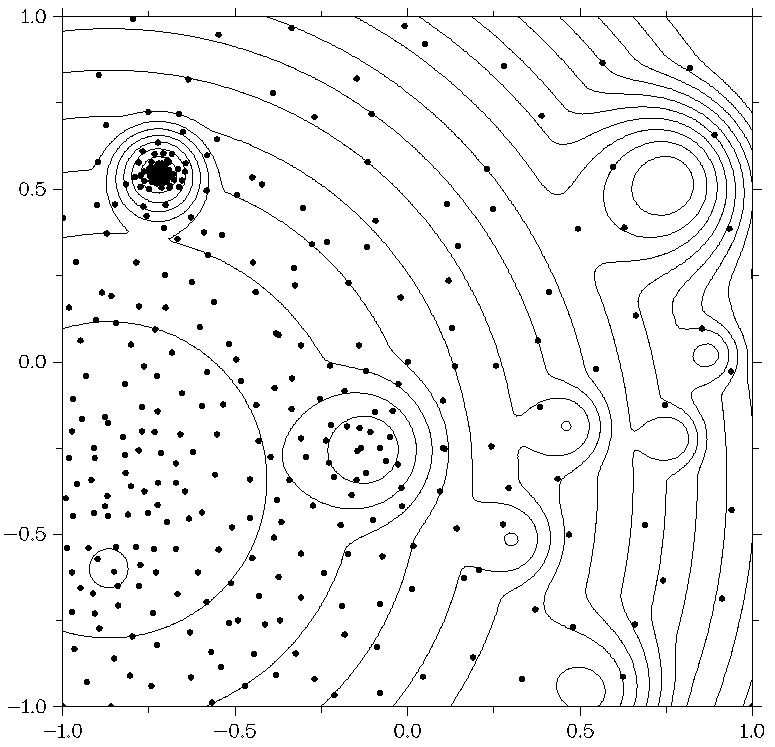
\includegraphics[width=0.75\textwidth]{fig2.jpg} 
  \caption{Minimization of a GKLS function of two variables by GSA}
  \label{fig:1}       % Give a unique label
\end{figure} 

The following theorem from \cite{Strongin2000} determines sufficient convergence conditions of the global search algorithm.

\textbf{Theorem}. Let the point $\overline{y}$ be the limit point of the sequence ${y^k}$ generated by the rules of GSA while minimizing the Lipschitzian with the constant $L$ function $\varphi(y), y \in D$. Then:
\begin{enumerate}
	\item If side by side with $\overline{y}$ there exists another limit point $y'$ of the sequence ${y^k}$ , then $\varphi(\overline{y})=\varphi(y')$.
	\item For any $k \geq 1$ $x^k=\varphi (y^k) \geq \varphi (\overline{y})$.
	\item If at some step of the search process the value $\mu$ from (\ref{eq:11}) satisfies the condition 
\[
  r\mu > 2^{3-1/N}L\sqrt{N+3},
\]
than $\overline{y}$ is a global minimizer of the function $\varphi (y)$ over $D$ and any global minimizer $y^\ast$ from () is also a limit point of the sequence ${y^k}$.
		
\end{enumerate}

\textbf{Remark}. As follows from the theorem, the limit points of the trial sequence ${y^k}$ generated by GSA are global minimizers. This property makes GSA substantially different from search techniques one way or another based on the random search concept which generates trial sequences everywhere dense in the search domain.


\section{Tuning the method for GENOPT problems}\label{sec:3}

The organizers of GENOPT competition have offered 18 classes of problems (see table \ref{tab:problems}, %new
where last two rows correspond to six classes of composite functions with $n=0,1,2$). In each class, 100 functions have been given.

\begin{table}
	\caption{The classes of problems to be solved within the competition}
	\label{tab:problems}
	\center
	\begin{tabular}{cccc}
		\hline\noalign{\smallskip}
		Index & Family & Type & Dimension \\
		\hline\noalign{\smallskip}
		0 &	 \multirow{6}{*}{GKLS} &	\multirow{2}{*}{non-differentiable} & 10 \\
		1 &	 &	 & 30 \\
		2 &	  &	\multirow{2}{*}{differentiable} & 10 \\
		3 &	 &	 & 30 \\
		4 &	  &	\multirow{2}{*}{twice differentiable} & 10 \\
		5 &	 &	 & 30 \\
		\hline\noalign{\smallskip}		
		6 &	\multirow{6}{*}{High condition}  &	\multirow{2}{*}{Rosenbrock} & 10 \\
		7 &	 &	 & 30 \\
		8 &	  &	\multirow{2}{*}{Rastrigin} & 10 \\
		9 &	 &	 & 30 \\
		10 &	  &	\multirow{2}{*}{Zakharov} & 10 \\
		11 &	 &	 & 30 \\
		\hline\noalign{\smallskip}
		$12+2n$ &	\multirow{2}{*}{Composite}  &	 & 10 \\
		$13+2n$ &	 &	 & 30 \\
\noalign{\smallskip}\hline
	\end{tabular}
\end{table}

The limit of 1 million computations of the function (trials) imposed by the organizers is essential for finding the global minimum of the functions with given dimensionalities. Thus, even for the 10-dimensional problems, having built a uniform grid with four points in each dimension, one goes already out of the 1 million points limit. %new
The global optimization algorithms that build non-uniform grid in the search domain put the points more efficiently. %new
However, for the 30-dimensional problems such an efficiency appears to be not enough as well. In this section, we describe four modifications of the core method used in solving various problems within the competition. The first two modifications have been applied to all problems, the third one – to the problems of GKLS class, and the last one has been used for solving the problems with Rastrigin, Rosenbrock, and Zakharov functions.

\subsection{Mixed global-local algorithm}\label{mixed}

One scheme aiming to accelerate the search process is to be outlined in this subsection (other schemes are described, for example, in \cite{Kvasov2006,Kvasov2015} ). The idea of acceleration is to magnify the characteristics of the intervals containing the best current estimates by introducing some factor depending on the function values estimated at the end-points of the corresponding interval. Following this idea, we introduce the modified characteristics 
\begin{equation}\label{eq:localR}
  R_\alpha(i) = \frac{R(i)}{\sqrt{(z_i-\varphi_k^\ast)(z_{i-1}-\varphi_k^\ast)}+\mu (1.5)^{-\alpha}},
\end{equation}
where $\mu$, $R(i)$ and $\varphi_k^\ast$ are respectively from (\ref{eq:11}), (\ref{eq:14}), (\ref{eq:phistar}), and $\alpha$ is some integer parameter for setting the desired level of localization. 

Next, it is possible to build a scheme \textit{mixing} the 'global' and the 'local' decision rules, i.e. switching between formulae (\ref{eq:14}) and (\ref{eq:localR}) in some systematic way. In our experiments we use \textit{global-to-local} ratio $q$, specifying the number of global trials preceding each local trial.

The mixed strategy has the following features. 	Firstly, both decision rules are based on the same information, so that each decision action (no matter local or global) uses the outcomes of all the trials performed. Secondly, non-stop global search assures the global convergence; the aim of the local refinement is to accelerate the attainment of low function values. 

Let us use a mixed global-local algorithm for solving a problem from section \ref{sec:1} with the global-to-local ratio $q=4$ and level of localization $\alpha = 15$. With this parameters the number of iterations was $203$. Fig.~\ref{fig:2} shows level lines of the same function from Fig.~\ref{fig:1} with points of the trials performed by the mixed method.

\begin{figure}
	\center
  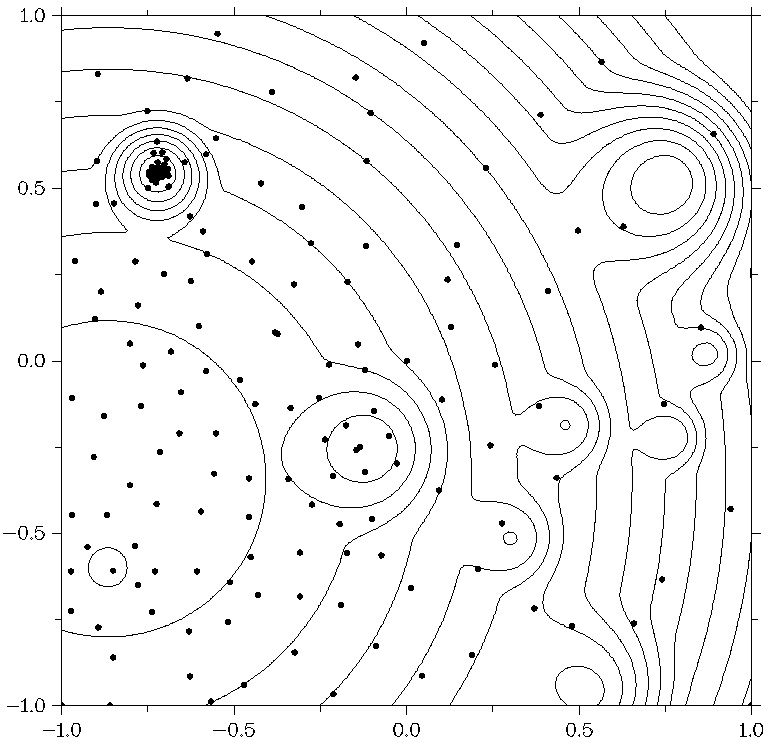
\includegraphics[width=0.75\textwidth]{fig3.jpg} 
  \caption{Minimization of a GKLS function of two variables by mixed GSA}
  \label{fig:2}       % Give a unique label
\end{figure} 

\subsection{Local refinement of the best current estimate} \label{hooke}

The second implemented modification of the core method consisted in a direct utilizing of a local optimization method, namely Hooke--Jeeves method \cite{HookeJeeves} (see also \cite{Wilde}, \cite{Himmelblau}). Schematically, the combined method works as follows:


\begin{itemize}
	\item The global phase
	
	\begin{itemize}
		\item Perform the GSA iterations until the current optimum (the minimal value of the objective function in the trial points computed already) is renovated.
	\end{itemize}
	
	\item The local phase
		\begin{itemize}
		\item Start Hooke-Jeeves method from the current optimum point with given exit condition according to precision.
		\item Add all the trial points of the local method into the GSA trial points database.
		\item Upon achieving given accuracy by the local method, go to the global phase.
	\end{itemize}

\end{itemize}


The accuracy of the local method (the termination condition) was taken as $10^{-5}$ for all problem classes of GKLS as well as for the Rastrigin and composite ones,  $10^{-7}$ for Rosenbrock functions, and $10^{-6}$ for Zakharov ones.

\subsection{Utilizing the random search for GKLS-30}\label{random}

The modification of the core method considered above have allowed solving almost all problems from the 10-dimensional GKLS classes (see more details in section \ref{sec:5}). However, these ones appeared to be insufficient for the 30-dimensional problems of this class. 
The multistart scheme was the next variant of the modification. Using Sobol quasi-random number generator, we have selected 500 start points. A local optimization method with the limitation not only in precision (stated above) but also in the number of iterations (1000) has been started in each point. Thus, 500 thousand trials could be spent in the local phase in the worst case. All the points of the trials executed at the local phase are stored in the database of the global method. Then, the global phase was started, when the rest of 1 million trials were executed using GSA.

\subsection{Use of separable search as an initial stage}\label{separable}

Since Rastrigin function is a separable one, one can search for its global optimum by performing the optimization in each coordinate separately. Thus, the following scheme has been employed in order to solve Rastrigin problem:


\begin{itemize}
	\item The separable stage 
	\begin{itemize}
		\item Select a start point.
		\item For each coordinate to perform:
		\begin{itemize}
			\item Fix all coordinated except the current one.
			\item Perform the optimization by one-dimensional GSA. 
		\end{itemize}
		\item Store all the trial points of the local method into the trial point database of GSA.		
	\end{itemize}
	\item The local stage 
	\begin{itemize}
		\item Start Hooke-Jeeves method with given exit condition according to precision from the point of current optimum.
		\item Store all the trial points of the local method into the trial point database of GSA.
		\item Upon achievement given precision by the local method, go to the global stage.
	\end{itemize}
\item The global stage
	\begin{itemize}
		\item Perform the iterations of GSA, until the current optimum (the minimum value of the objective function in the trial points computed already) is renovated.
	\end{itemize}	
\end{itemize}

The scheme considered above has allowed us to solve all the problems with 10-dimensional Rastrigin functions as well as with the 30-dimensional ones.

The same approach has been applied to solving the problems based on the unimodal functions (Rosenbrock and Zakharov ones) as well. In these cases, the separable stage provides a good initial approximation for the local method. Without the use of the separability, the local method starts from a point located far away from the global minimum and performs too many iterations until the termination conditions are satisfied. 

\section{Numerical experiments}\label{sec:5}

The methods considered in sections \ref{sec:1} and \ref{sec:3} and the modifications of these ones have been implemented in ExaMin solver intended for the parallel solving of the multidimensional multiextremal global optimization problems developed in Lobachevsky State University of Nizhni Novgorod. Global search algorithm and block nested optimization scheme \cite{Barkalov2014} make the algorithmic basis for ExaMin solver. According to the competition conditions, the sequential mode of the solver execution only has been used when solving the problems. However, ExaMin supports the systems with distributed memory (using MPI) as well as with shared memory (using OpenMP). Moreover, NVIDIA graphic processors and Intel Xeon Phi coprocessors are supported.

In the final stage of the competition, ExaMin solver has taken the 3rd prize in the overall ranking and the 1st one in the total number of the solved problems (fig.~\ref{fig:4}). The distribution of the classes of the solved tasks is presented in table \ref{tab:solved}. The parameter of the evolvents building was $m=10$. The parameter of the method was $r=2.5$ for all problems besides the ones from GKLS class. For GKLS, $r$ varied from 2.5 to 20.

\begin{figure}
	\center
  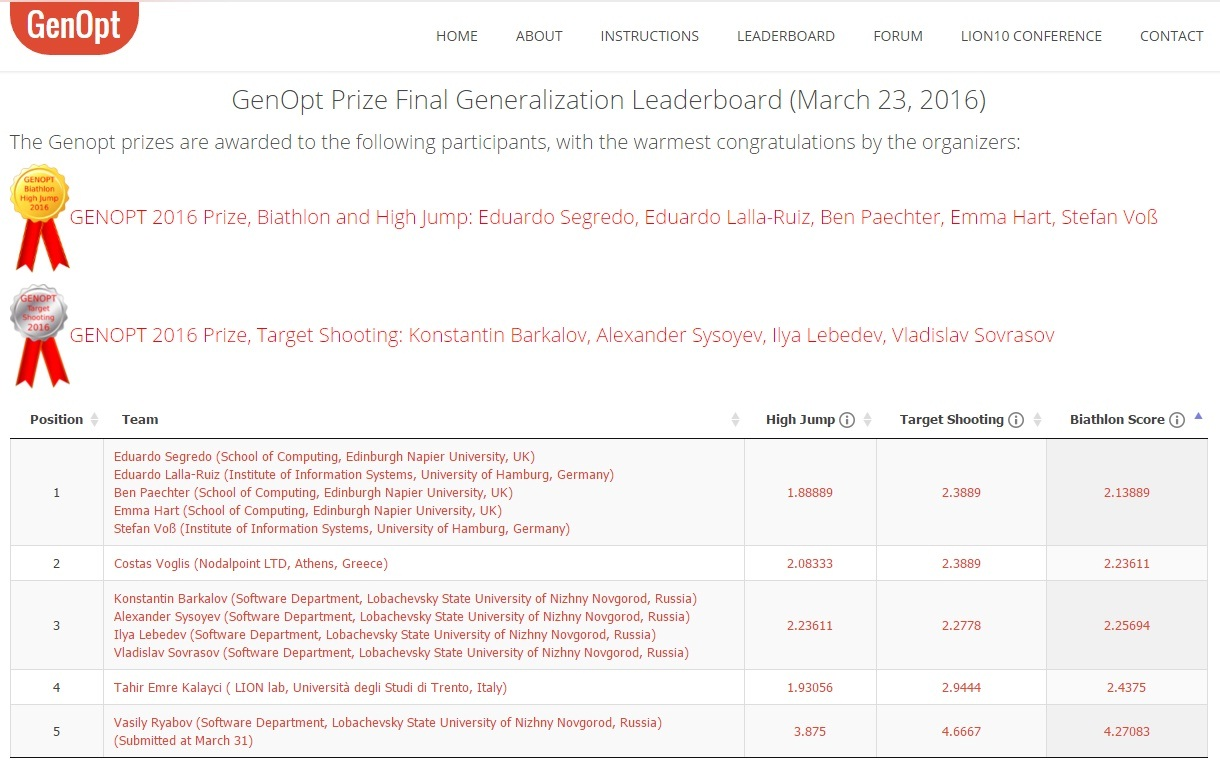
\includegraphics[width=1.00\textwidth]{fig4.jpg} 
  \caption{Final GENOPT leaderboard}
  \label{fig:4}       % Give a unique label
\end{figure} 

\begin{table}
	\caption{Total number of solved tasks from different classes}
	\label{tab:solved}
	\center
	\begin{tabular}{cc}
		\hline\noalign{\smallskip}
	Class & Tasks solved   \\
	\noalign{\smallskip} \hline \noalign{\smallskip}		
		GKLS--nd--10 & 99 \\
		GKLS--nd--30 & 15 \\
		GKLS--cd--10 & 96 \\
		GKLS--cd--30 & 1 \\
		GKLS--td--10 & 94 \\
		GKLS--td--30 & 0 \\
		Rosenbrock--10 & 100 \\
		Rosenbrock--30 & 100 \\
		Rastrigin--10 & 100 \\
		Rastrigin--30 & 100 \\
		Zakharov--10 & 100 \\
		Zakharov--30 & 100 \\
		Composite--10 & 100 \\
		Composite--30 & 100 \\
		\noalign{\smallskip}\hline
	\end{tabular}
\end{table}

The modification with the separable stage with the precision $0.02$ for the stop condition of one-dimensional GSA was used for all classes except GKLS. When solving the GKLS problems, the modifications from subsections \ref{mixed} and \ref{hooke} have been used first, then modification from subsection \ref{random} was applied. %new
The number of the solved problems with and without random search is presented in table \ref{tab:randsolved}.%new

\begin{table}
	\caption{Total number of solved tasks from different classes}
	\label{tab:randsolved}
	\center
	\begin{tabular}{ccc}
		\hline\noalign{\smallskip}
	Class &  \parbox[c]{3cm}{ \centering  Solved without\\random mode}   & \parbox[c]{3cm}{ \centering Solved with\\random mode}    \\
	\noalign{\smallskip} \hline \noalign{\smallskip}		
		GKLS--nd--10 & 78 & 99 \\
		GKLS--nd--30 & 0 & 15 \\
		GKLS--cd--10 & 67 & 96 \\
		GKLS--cd--30 & 0 & 1 \\
		GKLS--td--10 & 65 & 94 \\
		GKLS--td--30 & 0 & 0 \\
		\noalign{\smallskip}\hline
	\end{tabular}
\end{table}


\section{Conclusion}
In this work, the results of solving of the 10- and 30-dimensional problems of the unconditional global optimization from GenOpt 2016 competition are presented. The optimization methods used and the modifications of these ones directed onto the obtaining of a solution at given limitation of 1 million trials (computations of the objective function) are described. All the modifications considered are implemented in ExaMin solver employed in the conducting of the experiments. The numerical experiments have been carried out using Lobachevsky supercomputer \cite{Lobach}.

%\subsection{Acknowledgements}

\textbf{Acknowledgements.} This study was supported by the Russian Science Foundation, project No 15-11-30022 ``Global optimization, supercomputing computations, and applications''.

\begin{thebibliography}{99}
\bibitem{Hill}
Hill, J.D.: A search technique for multimodal surfaces. IEEE Transactions on Systems Science and Cybernetics. 5(1), 2--8 (1969)

\bibitem{Shekel}
Shekel J.: Test functions for multimodal search technique. Proceedings of the 5th Princeton Conference on Information Science Systems. Princeton, Princeton University Press. 354--359 (1971)

\bibitem{Strongin2000}
Strongin, R.G., Sergeyev, Ya.D.: Global optimization with non-convex constraints. Sequential and parallel algorithms. Kluwer Academic Publishers, Dordrecht (2000)

\bibitem{Barkalov2002}
Barkalov, K.A., Strongin, R.G.: A global optimization technique with an adaptive order of checking for constraints. Computational Mathematics and Mathematical Physics 42(9), 1289--1300 (2002)

\bibitem{Grishagin1978}
Grishagin, V.A.: Operation Characteristics of Some Global Optimization Algorithms. Problems
of Stochastic Search 7, 198--206 (1978) (in Russian)

\bibitem{Gaviano}
Gaviano, M., Kvasov, D.E, Lera, D., and Sergeyev, Ya.D.: Software for generation of classes of test functions with known local and global minima for global optimization. ACM Transactions on Mathematical Software 29(4), 469--480 (2003)

\bibitem{Kvasov2003}
Kvasov, D., Sergeyev, Ya.: Multidimensional global optimization algorithm based on adaptive diagonal curves. Computational Mathematics and Mathematical Physics 43(1), 40--56 (2003)

\bibitem{Sergeyev2013}
Sergeyev, Ya.D., Strongin, R.G., Lera, D.: Introduction to global optimization exploiting space-filling curves. Springer (2013)	

\bibitem{Sergeyev2010}
Lera D., Sergeyev Ya.D. Lipschitz and Holder global optimization using space-filling curves, Applied Numerical Mathematics, 60(1-2), 115--129 (2010)

\bibitem{Sergeyev1994}
Sergeyev, Ya.D., Grishagin, V.A.: A parallel method for finding the global minimum of univariate functions. J. Optim. Theory Appl. 80(3), 513--536 (1994)

\bibitem{SergeyevGrishagin}
Sergeyev, Ya.D., Grishagin, V.A.:  Sequential and parallel global optimization algorithms. Optimization Methods and Software. 3, 111--124 (1994)

\bibitem{Gergel1996}
Gergel, V.P.: A method of using derivatives in the minimization of multiextremum functions. Computational Mathematics and Mathematical Physics 36(6), 729--742 (1996)

\bibitem{Gergel1997}
Gergel, V.P.: A global optimization algorithm for multivariate functions with lipschitzian first derivatives. J. Glob. Optim. 10(3), 257--281 (1997)

\bibitem{Grishagin1997}
Grishagin, V.A., Sergeyev, Ya.D., Strongin, R.G.: Parallel characteristical algorithms for solving problems of global optimization. J. Glob. Optim. 10(2), 185--206 (1997)

\bibitem{Gergel1999}
Gergel, V.P., Sergeyev, Ya.D.: Sequential and parallel algorithms for global minimizing functions with Lipschitzian derivatives. Computers and Mathematics with Applications, 37(4-5), 163--179 (1999)

\bibitem{Grishagin2001}
Sergeyev Ya.D, Grishagin V.A.: Parallel asynchronous global search and the nested optimization scheme. Journal of Computational Analysis and Applications. 3(2), 123--145 (2001)

\bibitem{Strongin2003}
Strongin, R.G., Sergeyev, Ya.D.: Global optimization: fractal approach and non-redundant parallelism. J. Glob. Optim. 27(1), 25--50 (2003)

\bibitem{Gergel2005}
Gergel, V.P., Strongin, R.G.: Parallel computing for globally optimal decision making on cluster systems. Future Generation Computer Systems, 21(5), 673--678 (2005)

\bibitem{Barkalov2013}
Barkalov, K., Polovinkin, A., Meyerov, I., Sidorov, S., Zolotykh, N.: SVM regression parameters optimization using parallel global search algorithm. Lecture Notes in Computer Science. 7979, 154--166 (2013)

\bibitem{Barkalov2014} 
Barkalov, K.A., Gergel, V.P.: Multilevel scheme of dimensionality reduction for parallel global search algorithms. Proceedings of the 1st International Conference on Engineering and Applied Sciences Optimization -- OPT-i 2014. pp. 2111--2124. (2014)

\bibitem{Grishagin2015} 
Gergel, V., Grishagin, V., Israfilov, R.: Local tuning in nested scheme of global optimization. Procedia Computer Science, 51(1), pp. 865--874. (2015)

\bibitem{Gergel2015} 
Gergel, V., Grishagin, V., Gergel, A.: Adaptive nested optimization scheme for multidimensional global search. Journal of Global Optimization, 17 p. Article in Press. (2015)

\bibitem{Barkalov2016} 
Barkalov, K., Gergel, V.: Parallel global optimization on GPU. Journal of Global Optimization. 18 p. Article in Press. (2016) 

\bibitem{Kvasov2006} 
Sergeyev, Ya.D., Kvasov D.E.: Global search based on efficient diagonal partitions and a set of Lipschitz constants. SIAM Journal on Optimization, 16(3), 910--937 (2006)

\bibitem{Kvasov2015} 
Paulavicius, R., Sergeyev, Y., Kvasov, D., Zilinskas, J. Globally-biased DISIMPL algorithm for expensive global optimization, Journal of Global Optimization, 59(2-3), 545--567 (2015).

\bibitem{HookeJeeves} 
Hooke, R., Jeeves, T.A.: "Direct search" solution of numerical and statistical problems // Journal of the ACM. 8(2), 212--229 (1961)

\bibitem{Wilde} 
Wilde, D.J.: Optimum Seeking Methods. Prentice-Hall, Engelwood Cliffs, New Jersey (1964)

\bibitem{Himmelblau} 
Himmelblau, D.M.: Applied Nonlinear Programming. McGraw-Hill, New York (1972)

\bibitem{Lobach}
\url{http://www.top500.org/system/178472}


                                                                           
\end{thebibliography}

\end{document}